\documentclass{article}
\usepackage[utf8]{inputenc}
\usepackage{amssymb}

\title{Resumen Química I}
\author{}
\date{}

\usepackage{amsmath,amsfonts,amssymb,amsthm}
\usepackage{natbib}
\usepackage{graphicx}
\usepackage[margin=1.0in]{geometry}

%%\newcommand{comando kliao}{comando bueno}
\DeclareMathOperator\cis{cis}
\DeclareMathOperator\Arg{Arg}

\begin{document}
\maketitle


\section{Clase 1}


\subsection{Naturaleza ondulatoria de la luz}
La luz que vemos con nuestros ojos, la luz visible, es un tipo de \textbf{radiación electromagnética} (es la emisión y transmisión de energía de forma de \textbf{ondas electromagnéticas})

\subsubsection{Ondas}
Una onda es una alteración vibracional mediante la cual se transmite la energía.
\begin{itemize}
    \item \textbf{Longitud de onda}: ($\lambda$, lambda) es la longitud entre puntos iguales de ondas sucesivas. (m, cm, o nm)
    \item \textbf{Amplitud}: es la longitud vertical desde la linea media de una onda a su cresta o a su valle.
    \item \textbf{Frecuencia}: ($f$ o $v$) es el número de ondas que pasan por un punto particular en un segundo. (Hz)
\end{itemize}
La \textbf{rapidez} es otra de las propiedades importantes de una onda, que depende del tipo de onda y del medio en el cual viaja (por ejemplo, aire, agua o vacío). En general la rapidez de una onda está dada por
\begin{equation}
    v=\lambda \cdot f
\end{equation}

\subsubsection{Ondas electromagnéticas}
Una \textbf{onda electromagnética} es una alteración energética compuesta por un componente de campo eléctrico y un componente de campo magnético. Dado que la rapidez o velocidad de una onda es el producto de la longitud ($\lambda$) por su frecuencia ($f$). Para una onda electromagnética se cumple
\begin{equation} \label{clambdaf}
    c=\lambda \cdot f
\end{equation}
Las ondas electromagnéticas viajan en el vacío a una velocidad constante de $3.00\times 10^8 $m/s. Velocidad también conocida como \textbf{velocidad de la luz}

\subsection{El espectro electromagnético}
La radiación electromagnética es la emisión y transmisión de energía en forma de \textbf{Ondas electromagnéticas}. El espectro electromagnético muestra los \textbf{diferentes tipos de radiación electromagnética}.
De mayor a menor frecuencia (menor a mayor $\lambda$) van en el siguiente orden: Rayos gamma, Rayos X, Ultravioleta, Lux visible, Infrarrojo, Microondas, Ondas de radio.
Notemos que la luz visible va de 400nm (rojo) a 700nm (azul).
Para calcular la frecuencia o longitud de onda se utiliza la ecuación \ref{clambdaf}, ya que el valor de la velocidad es igual si se está en el vacío.


\subsection{Radiación de cuerpo oscuro}
La cantidad de energía radiante de cierta longitud de onda emitida por un objeto depende de su temperatura. Antes no se entendía la relación entre la temperatura, la intensidad y la longitud de onda de la radiación emitida.

\subsection{Teoría cuántica de Planck}
La teoría de Planck propone que la radiación electromagnética solo puede ser liberada (o absorbida) por los átomos en "paquetes" discretos de tamaño mínimo o \textbf{cuanto} (que significa cantidad fija).
En general, la energía ($E$), de un solo cuanto es igual a una constante ($h$) multiplicada por su frecuencia ($f$)
\begin{equation}
    E=h\cdot f
\end{equation}
$E$: energía de un solo cuanto.
$h$: \textbf{Constante de Planck} $=6.63\times 10^{-34}J\cdot s$.
Dado que $f=\frac{c}{\lambda}$, entonces:
\begin{equation}
    E=h\frac{c}{\lambda}
\end{equation}

\subsection{Efecto fotoeléctrico}
El \textbf{efecto fotoeléctrico} es el fenómeno en el que los electrones son expulsados desde la superficie de ciertos metales que se han expuesto a la luz de al menos una determinada frecuencia mínima (frecuencia umbral). Quien dio explicación a este fenómeno fue Albert Einstein, lo que le valió un premio nobel en 1921.
Los electrones de mantienen unidos en el metal por fuerzas de atracción y para emitirlos, se necesita que un fotón tenga una energía suficientemente alta para sacarlos (frecuencia umbral de la luz), la que está dada por la ecuación de Planck.
Si se hace incidir en el metal luz con una frecuencia mayor a la umbral, los electrones no sólo serán emitidos, tambien adquirirán cierta energía cinética ($E_c$).

En la ecuación $E_c$ es la energía cinética del electrón emitido y $W$ es la función del trabajo, que es una medida de cuán fuerte están unidos los electrones en el metal.

\section{Clase 2}

\subsection{Espectro de líneas de absorción y emisión}
Un \textbf{espectro} es la separación de la radiación electromagnética en sus diferentes componentes de longitud de onda diferente. Los \textbf{espectros de emisión}, son los espectros continuos o de líneas de radiación emitida por las sustancias. Los \textbf{espectros de absorción}, son creados por la absorción selectiva de radiación por las sustancias. 
Los elementos absorben energía de la misma longitud de onda a la que emiten.

\subsection{La ecuación de Rydberg}
\textbf{Johann Balmer} planteó una ecuación empírica que explicaba las líneas observables del espectro del hidrógeno
\begin{equation}
    f=3.29\times 10^{15}s^{-1}(\frac{1}{2^2}-\frac{1}{n^2})
\end{equation}
\textbf{Johannes Rydberg} propuso una ecuación general que explicaba todas las líneas espectrales del hidrógeno.
\begin{equation}
    \frac{1}{\lambda}=R_H(\frac{1}{n_{i}^{2}}-\frac{1}{n_{f}^{2}})
\end{equation}
$\lambda$: longitud de onda.
$R_H$: constante de Rydberg ($1.096776\times 10^7 m^{-1}$).
$n_{i(\text{inicial})}$ y $n_{f(\text{final})}$: enteros positivos donde $n_2>n_1$.

\subsection{El modelo atómico de Bohr}
\begin{itemize}
    \item Los $e^-$ giran alrededor del núcleo del átomo con energía constante.
    \item Las órbitas son circulares y están cuantizadas en energía.
    \item Las órbitas cercanas al núcleo son de menor energía y las más lejanas de mayor energía.
    \item Si un $e^-$ absorbe energía, este se puede promover a un nivel de mayor energía (estado excitado).
    \item Cuando el $e^-$ regresa a un nivel menor de energía, emite energía (fotones).
\end{itemize}
Energía de la transición electrónica (\textbf{importante})

\begin{equation}
    E=hf=R_H(\frac{1}{n_{i}^{2}}-\frac{1}{n_{f}^{2}})
\end{equation}
$R_H=2.18 \times 10^{-18}J$.
$n=$ número cuántico principal

La transición de un $e^-$ entre niveles de energía involucra la emisión o absorción de un fotón de frecuencia $f$ y energía $hf$.

\subsubsection{Limitaciones del modelo atómico de Bohr}
\begin{enumerate}
    \item Los electrones sólo existen en ciertos niveles discretos de energía descritos con números cuánticos.
    \item El movimiento de un electrón de un nivel a otro involucra la absorción o liberación de energía.
\end{enumerate}
\textbf{Limitaciones:}
\begin{itemize}
    \item El modelo de Bohr ofrece una explicación al espectro de líneas del átomo de hidrógeno. Sin embargo, \textbf{no puede explicar los espectros de otros átomos}, o sólo lo hace de manera muy limitada.
    \item El modelo de Bohr \textbf{ignora las propiedades ondulatorias} del electrón.
\end{itemize}


\section{Clase 3}
\subsection{Postulado de Broglie}
"Si las ondas luminosas se comportan como una corriente de partículas (fotones), quizá partículas como los electrones tengan propiedades ondulatorias".
Propuso que los electrones, al igual que los fotones (cuantos de energía) se comportan como partículas (masa) y ondas (energía).
Los electrones se comportan como ondas estacionarias que ondulan en posiciones fijas.
\begin{equation}
    \lambda=\frac{h}{mv}
\end{equation}
$\lambda:$ la longitud de onda asociada a la partícula (\textbf{normalmente hay que transformar a nanómetros}).
$m:$ masa de la partícula.
$v:$ rapidez de la partícula.

\textbf{Lester y Clinton Davisson} (físicos americanos) demostraron que los electrones poseen propiedades ondulatorias. Al dirigir un rayo de electrones sobre una delgada lámina de oro.
%%%%% ver que wea hizo G.P Thomson el de la foto que aparece en la pagina 6/30

\subsection{Principio de incertidumbre de Heinsenberg}
La naturaleza dual de la materia impone una limitación fundamental a la precisión con que podemos conocer un tanto la posición, como la trayectoria (momentum) de cualquier objeto.
"Es imposible conocer con certeza el momento p (definido como la masa por la rapidez) y la posición de una partícula simultaneamente"
\begin{equation}
    \Delta x \Delta p \geq \frac{h}{4\pi}
\end{equation}
$\Delta x:$ incertidumbre en la posición.
$\Delta p=mv:$ incertidumbre en el momento.

\subsection{La ecuación de Schrödinger}
La ecuación de Schrödinger involucra el comportamiento de una \textbf{partícula}, en términos de la \textbf{masa (m)}, y el de \textbf{onda} en términos de una \textbf{función de onda} ($\Psi$, psi) que depende de la ubicación del sistema en el espacio.
\begin{equation}
    \frac{d^2\Psi}{dx^2} + \frac{d^2\Psi}{dy^2} + \frac{d^2\Psi}{dz^2} + \frac{8\pi^2m}{h^2}(E-V)\Psi=0
\end{equation}
La función de onda ($\Psi$) en sí misma no tiene un significado físico directo, el cuadrado de ella ($\Psi^2$) representa la probabilidad de encontrar al electrón en una cierta región del espacio.

\subsection{Orbitales atómicos y números cuánticos}
La ecuación de Schrödinger produce un conjunto de funciones, que representan zonas del espacio tridimensional donde hay mayor probabilidad de encontrar al electrón. Estas funciones de onda se denominan \textbf{orbitales}.
Un \textbf{orbital atómico} se considera como la función de onda del electrón de un átomo.
En la ecuación de Schrödinger los orbitales atómicos están descritos por un conjunto de números llamados \textbf{números cuánticos}.
Son parámetros numericos que derivan de la ecuación de Schrödinger y describen la distribución de los electrones en el átomo.
Se necesitan \textbf{4 números cuánticos} para describir los orbitales atómicos:
\begin{itemize}
    \item Número cuántico principal ($n$)
    \item Número cuántico de momento angular ($l$)
    \item Número cuántico magnético ($m_l$)
    \item Número cuántico de spin electrónico ($m_s$)
\end{itemize}

\subsubsection{Número cuántico principal}
\begin{itemize}
    \item Puede tomar \textbf{solo} valores enteros (1, 2, 3, etc). Cada valor de $n$ designa un nivel o capa.
    \item Determina la \textbf{energía} del electrón. Cuanto mayor sea el valor de $n$, mayor la energía del electrón.
    \item Es una medida del tamaño del orbital y se relaciona con la \textbf{distancia promedio} del electrón al núcleo en determinado orbital.
    \item A mayor valor de $n$, mayor es la distancia respecto al núcleo, por lo tanto el orbital es más grande.
\end{itemize}

\subsubsection{Número cuántico de momento angular}
Este número expresa la \textbf{forma} de los orbitales. Los valores de $l$ dependen del valor del número cuántico principal $n$, segun $l=n-1$.

%% ver si se puede agregar la tabla que aparece en la pagina 18/30

\subsubsection{Número cuántico magnético}
\begin{itemize}
    \item Describe la \textbf{orientación} del orbital en el espacio.
    \item Indica el número de orbitales presentes en un subnivel con cierto valor de $l$.
    \item Depende del valor de $l$ según $m_l=2l+1$
    \item su valor varia desde $-l$ hasta $+l$, pasando por 0.
    
\end{itemize}

%%ver si se puede agregar la tabla de la pagina 19/30

\subsubsection{Número cuántico de spin electrónico}
Representa el giro del electrón sobre su propio eje (espín) y puede tener dos valores de $+\frac{1}{2}$ ó $-\frac{1}{2}$.

\subsection{Forma y orientación de los orbitales atómicos}
\subsubsection{Orbitales s}
Los orbitales s son esféricos
%agregar mas weas%

\subsubsection{Orbitales p}
Están conformados por 2 segmentos lobulares, los orbitales p son perpendiculares entre si, con orientaciones ($p_x,p_y,p_z$). Estos 3 orbitales tienen el mismo tamaño, forma y energía, sólo cambia su orientación. Los orbitales p comienzan con el número cuántico principal $n=2$, ya que
para $n=2$, $l=1$.

\subsubsection{Orbitales d}
En total hay 5 orbitales d para un valor determinado de $l$. Estos orbitales comienzan con el número cuántico principal $n=3$, ya que para $n=3$, $l =2$.
%% verificar si esta wea de los orbitales esta bien escrita

\subsubsection{Orbitales f}
Hay 7 orbitales f para un valor determinado de l. Estos orbitales comienzan con el número cuántico principal $n=4$, ya que
para $n=4$, $l =3$.


\begin{figure}[h]
\caption{Resumen de orbitales atómicos}
\centering
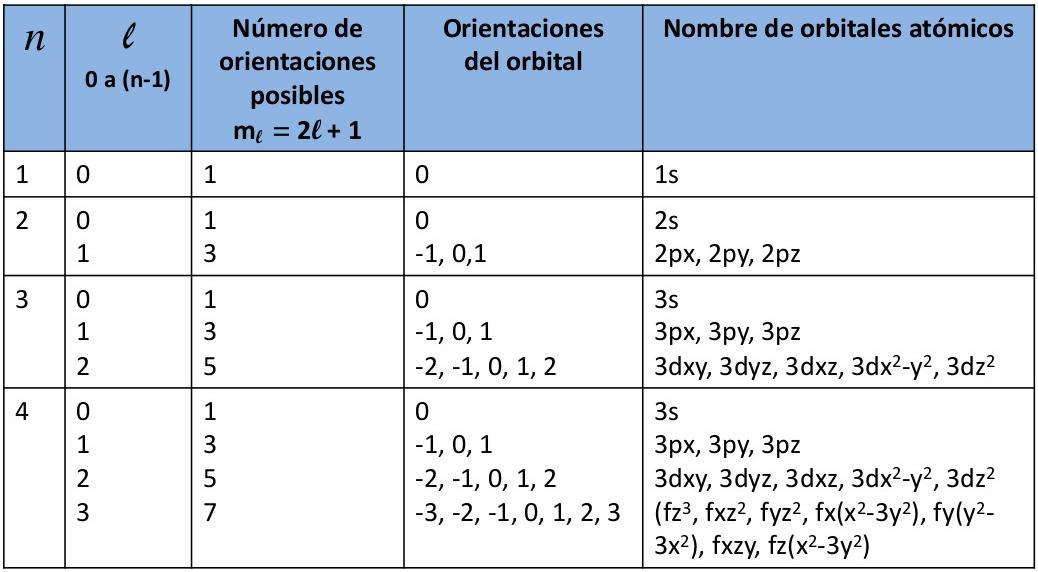
\includegraphics[scale=0.4]{imagenes/tabla1.jpg}
\end{figure}

\section{Clase 4}
\subsection{Configuración electrónica}

\subsection{Principio de exclusión de Pauli}
El principio de exclusión de Pauli establece que no es posible que dos electrones de un átomo tengan los mismos cuatro números cuánticos.

\subsection{Regla de Hund}
La regla de Hund establece que la distribución electrónica más estable en los subniveles es la que tiene el mayor número de espines paralelos.

\subsection{Principio de Aufbau}
El principio de Aufbau (construcción en alemán) establece que cuando los protones se incorporan al núcleo de uno en uno para construir los elementos, los electrones se suman de la misma  forma a los orbitales atómicos.

\subsection{Como realizar una configuración electrónica}
\begin{enumerate}
    \item Determinar el número de electrones que tiene el átomo, para un átomo neutro es igual a \textbf{Z}.
    
    \item Ubicar los electrones en cada uno de los niveles y subniveles de energía, comenzando por el más cercano al núcleo ($n=1$), según la regla de las diagonales.
\end{enumerate}

\begin{figure}[h]
\caption{Diagrama de las diagonales}
\centering
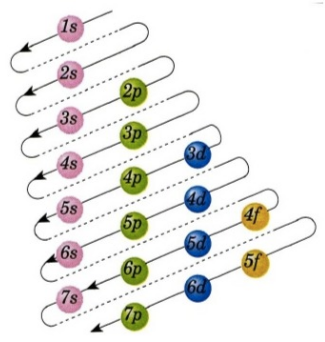
\includegraphics[scale=0.4]{imagenes/imagen1.png}
\end{figure}

%%%%%%

\subsection{Configuraciones abreviadas}
Al escribir la configuración electrónica abreviada de un elemento, la configuración electrónica del gas noble de número atómico más cercano pero menor, se representa con su símbolo químico encerrado en corchetes.

\section{Clase 5}

\section{Clase 6}

\section{Clase 7}


\end{document}